\documentclass[handout,t,compress]{beamer}
\usetheme{Singapore}

\sloppy
%\usepackage[scaled]{helvet}
%\usepackage{eulervm}

\usepackage{multicol}
\usepackage{fp-eval}
\usepackage{hyperref}
\usepackage{fancyvrb}
%\usepackage{pstricks,pst-node,pst-tree,pst-plot,pst-3dplot,multido}
\usepackage{graphicx}

\usepackage{alltt}


\newcommand{\bframe}[1]{\begin{frame}[fragile]\frametitle{#1}}

\newcommand{\bbnf}{\begin{center}\begin{tabular}{rcl}}
\newcommand{\bnf}[2]{#1 & ::= & #2 \\}
\newcommand{\ebnf}{\end{tabular}\end{center}}

\newcommand{\myskip}{\vspace{-1em}\hrulefill}
\newcommand{\myrule}[1]{\vspace{-1ex}\centerline{\rule{#1cm}{1pt}}}
\newcommand{\myline}[1]{\centerline{#1}}
\newcommand{\bkt}[1]{\ensuremath{\langle\mbox{#1}\rangle}}
\newcommand{\br}{\mbox{~}|\mbox{~}}

\definecolor{orange}{rgb}{1,.5,0}
\definecolor{pink}{rgb}{1,.75,.75}
\definecolor{ltblue}{rgb}{.75,.75,1}

\newcommand{\be}{\begin{eqnarray*}}
\newcommand{\ee}{\end{eqnarray*}}

\newcommand{\bi}{\begin{itemize}}
\newcommand{\li}{\item}
\newcommand{\ei}{\end{itemize}}

\newcommand{\grph}[2]{
\begin{columns}
\column{0.01\textwidth}
\column{0.6\textwidth}
\begin{pspicture}[showgrid=#1](-2,-2)(5,5)
#2
\end{pspicture}
}

\newcommand{\txt}[1]{
\column{0.4\textwidth}
\rput[bl](0,0){\parbox{\textwidth}{
\footnotesize
\begin{itemize}
#1
\end{itemize}}}
\end{columns}}


\AtBeginSection[]
{
\bframe{Outline}
\tableofcontents[currentsection]
\end{frame}
}

\title{Simple Soccer}
\subtitle{A game demo from {\em Programming Game AI by Example}, Mat Buckland}
\author{CSCI 321}
\institute{WWU}

\begin{document}\small

\bframe{~}
\titlepage
\end{frame}

\bframe{Simple Soccer}
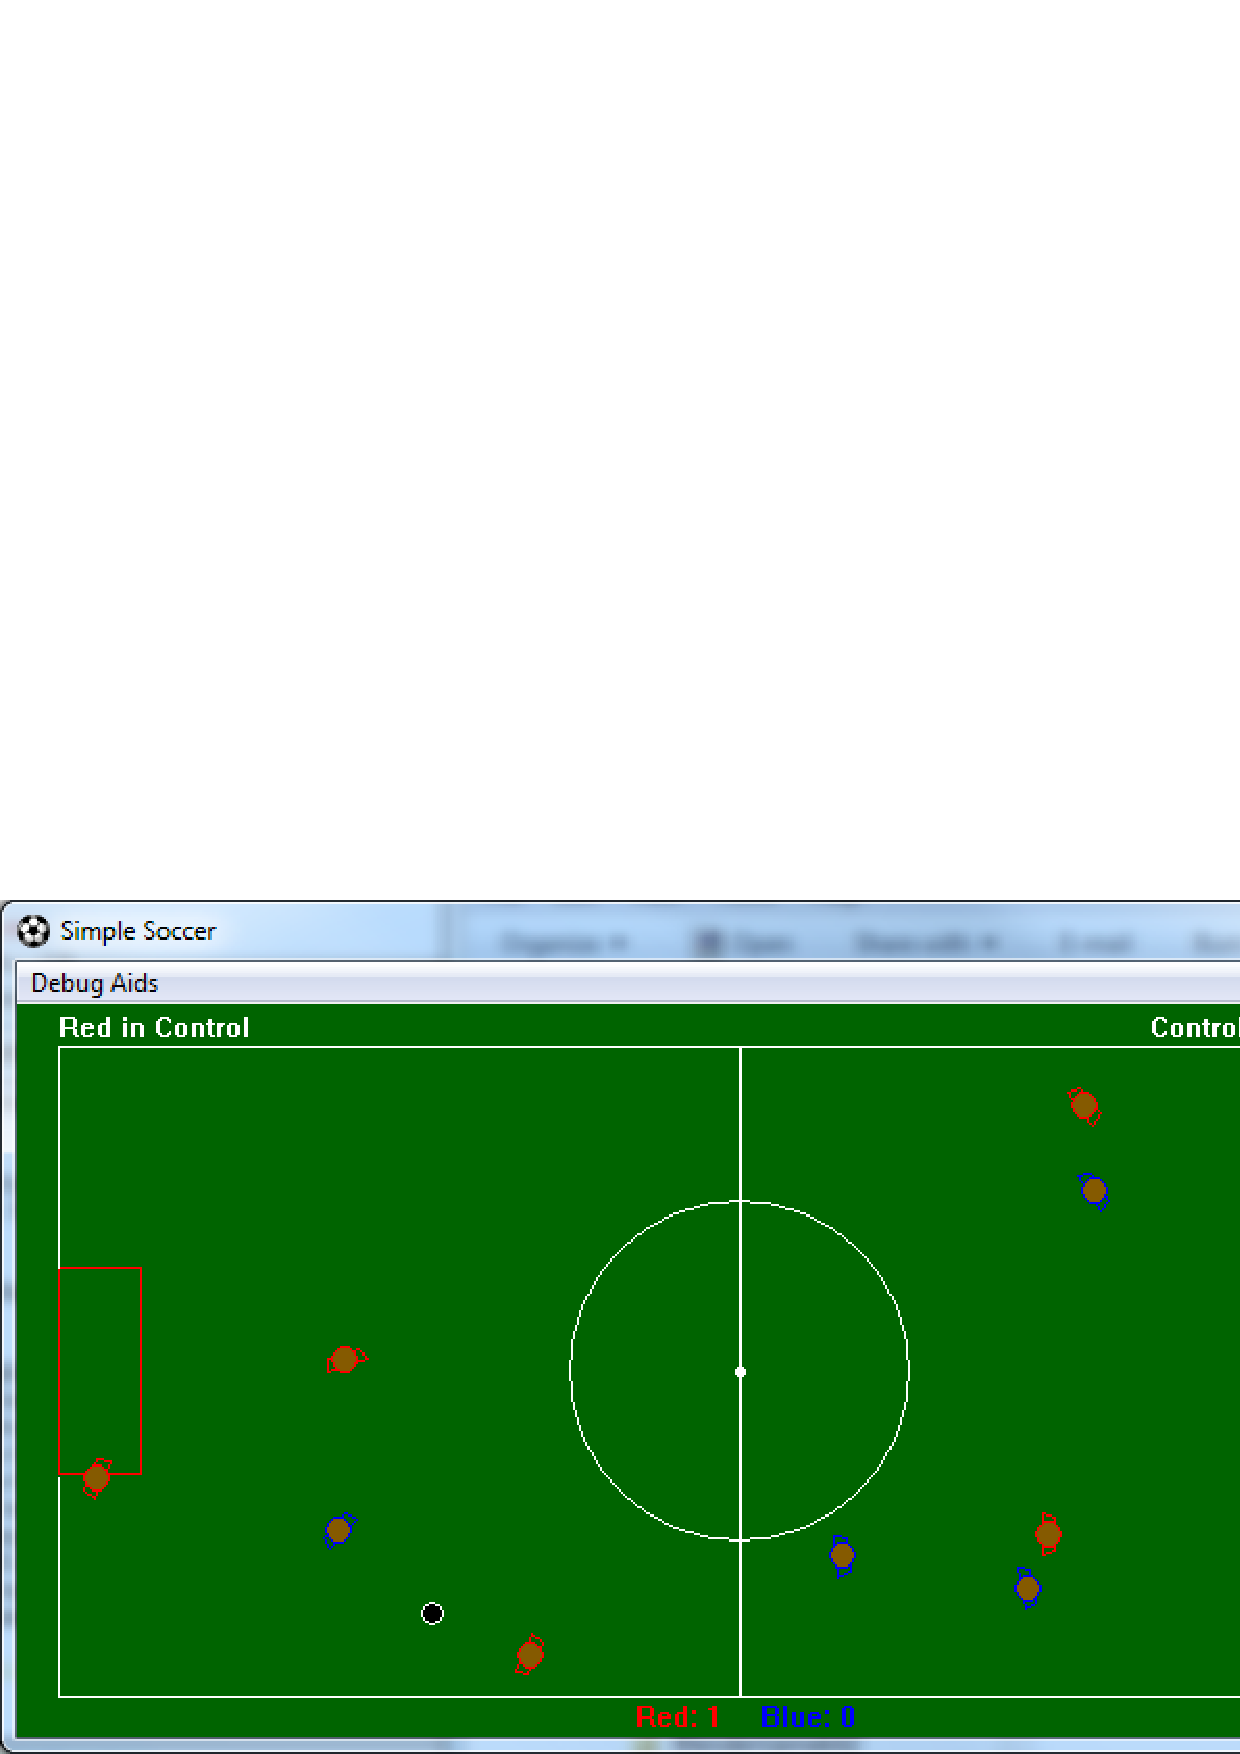
\includegraphics[scale=0.4]{simplesoccergame.png}
\end{frame}

\bframe{Simple Soccer}
\begin{itemize}
\item Soccer pitch
\item Goals
\item Ball
\item Teams
\item Field players
\item Goalies
\end{itemize}
\end{frame}

\bframe{Pitch}
\begin{itemize}
\item  Holds center spot for game restart.
\item Booleans:  {\tt GameOn}, {\tt GoalieHasBall}
\end{itemize}
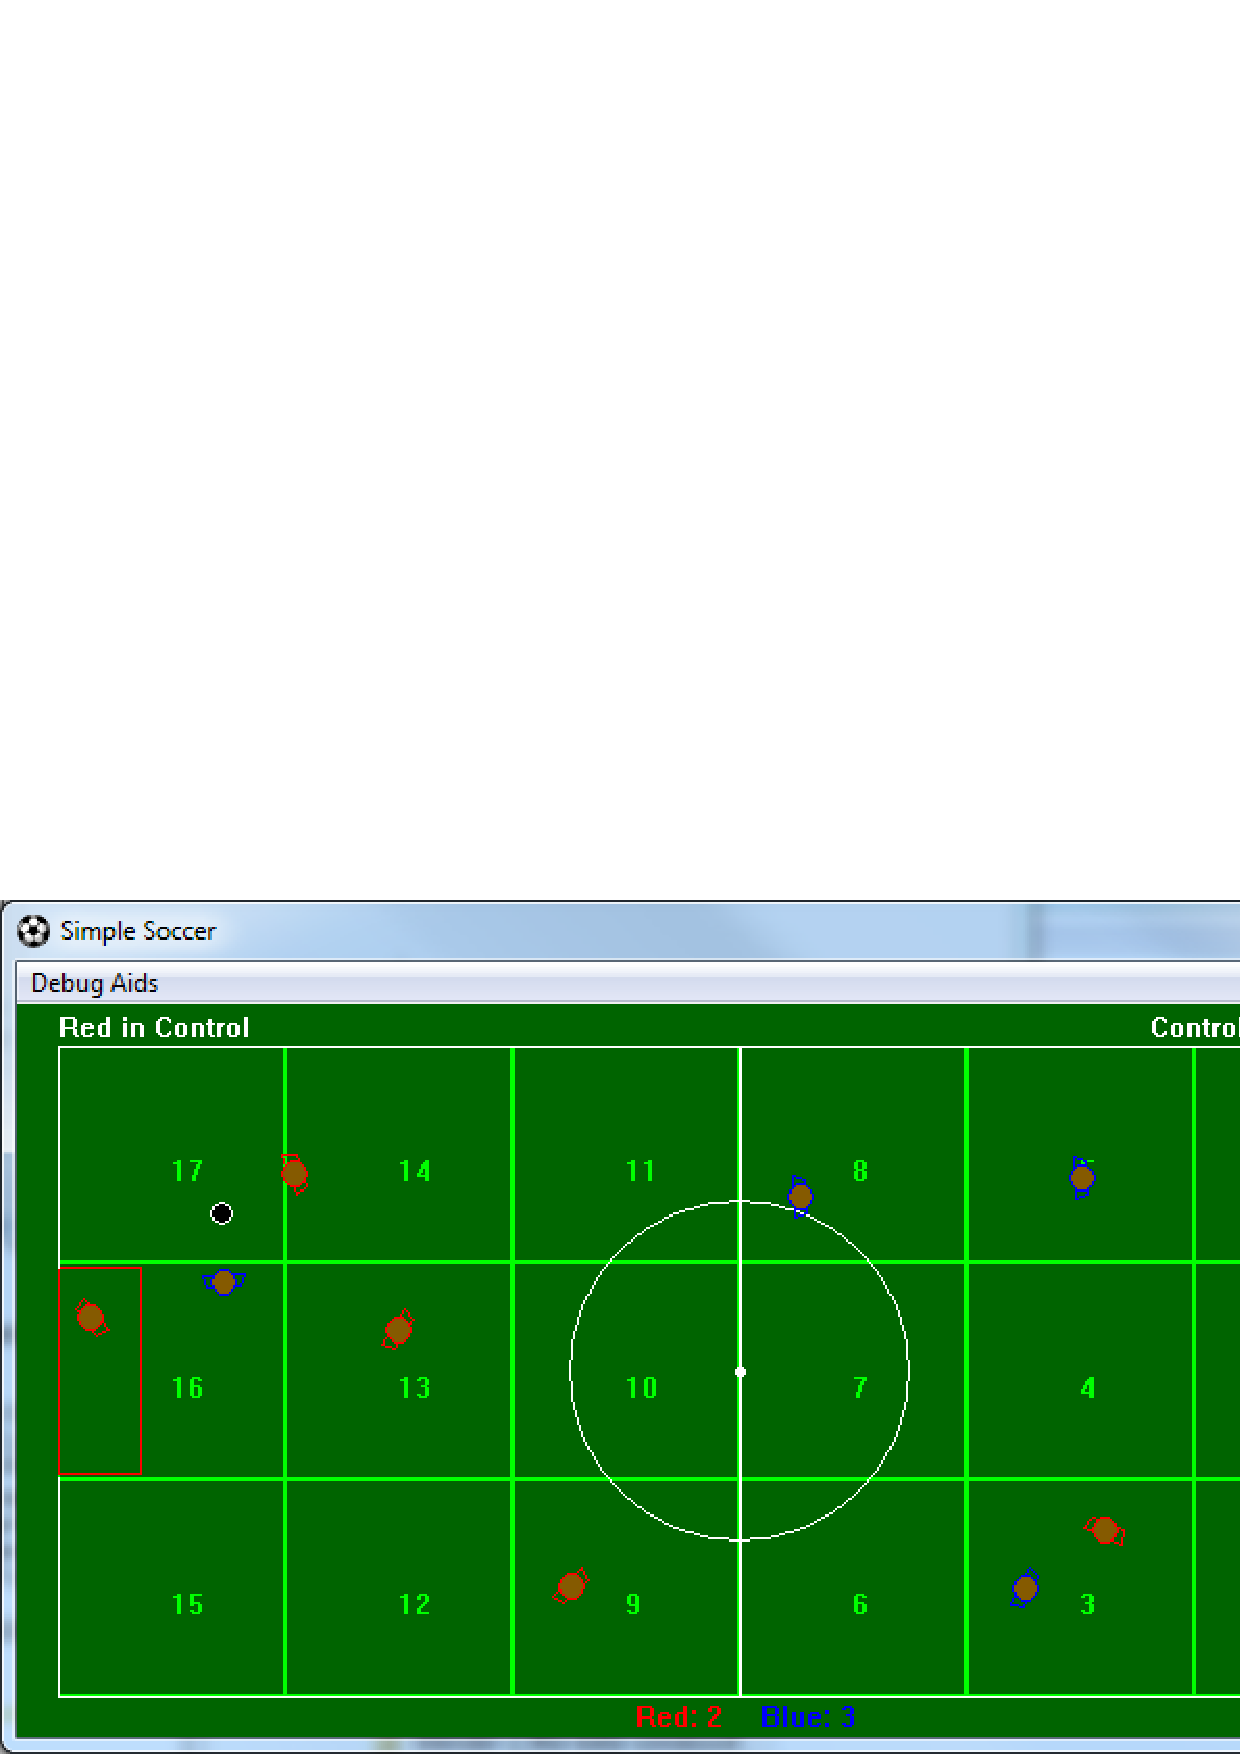
\includegraphics[scale=0.4]{simplesoccerregions.png}
\end{frame}

\bframe{Pitch divided into regions}
\begin{itemize}
\item Players head for home region if nothing else to do.
\item Home region may change during play.
\end{itemize}
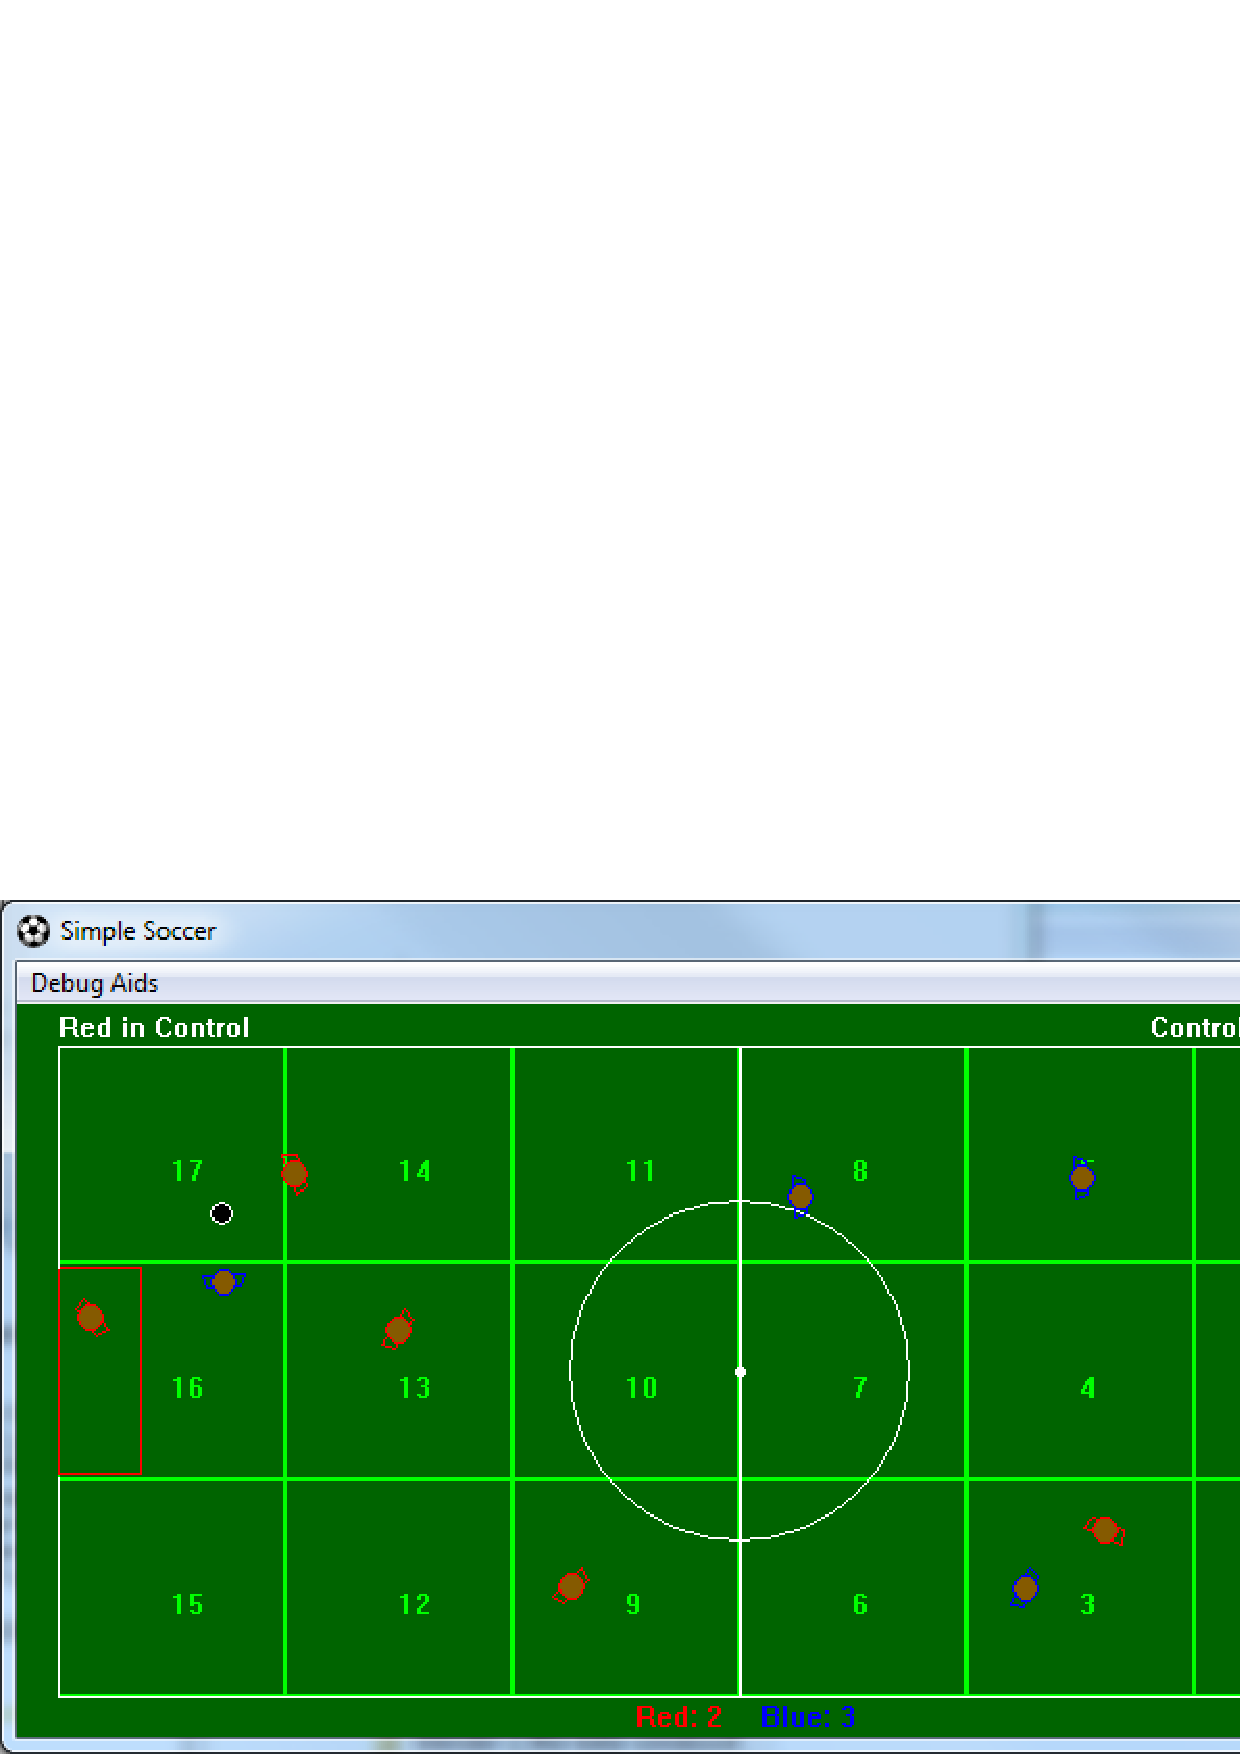
\includegraphics[scale=0.4]{simplesoccerregions.png}
\end{frame}

\bframe{Goals}
\begin{itemize}
\item Checks for score (collision with ball).
\item Keeps score, resets game.
\end{itemize}
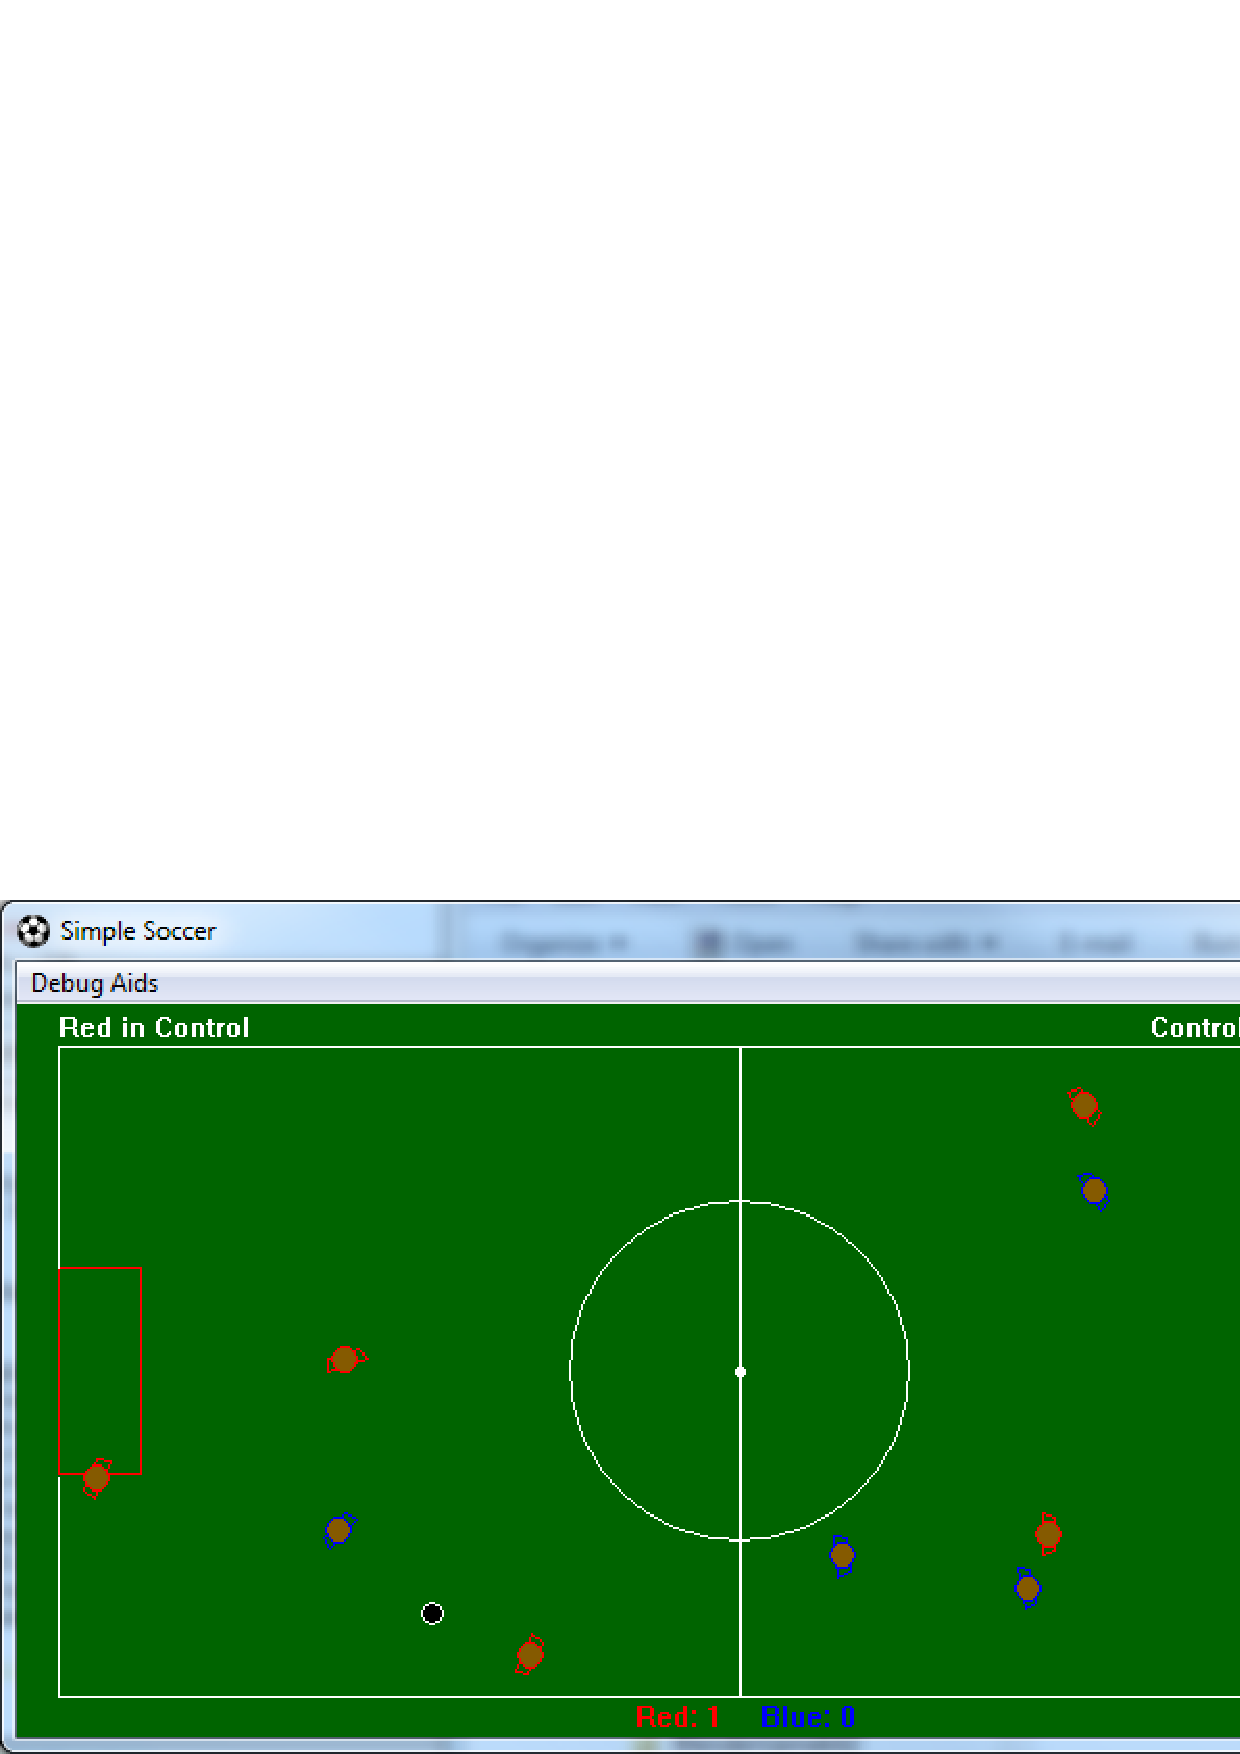
\includegraphics[scale=0.4]{simplesoccergame.png}
\end{frame}

\bframe{Ball}
\begin{itemize}
\item Checks for collisions with boundary
\item Does not collide with players (need to dribble)
\item Accelerated by kick, decelerated by friction. 
\item Players need to make predictions:
\begin{itemize}
\item {\tt FuturePosition}:
\[
\Delta x = u\Delta t + \frac{1}{2}a\Delta t^2
\]
 $\Delta x$ is
  distance traveled, $\Delta t$ is time taken.
\item {\tt TimeToCoverDistance}:
\begin{eqnarray*}
\Delta t &=& \frac{v-u}{a}\\
v &=& \sqrt{u^2 + 2a\Delta x}
\end{eqnarray*}
$u$ is the starting velocity, $v$ is the ending velocity
\end{itemize}
\item Velocities are not accumulative, but that works for this game.
\end{itemize}

\end{frame}

\bframe{Soccer Team}
\begin{itemize}
\item A {\em tiered} or {\em hierarchical} AI, some decisions handled
  at the team level, some at individual level.
\begin{itemize}
\item Used in RTS: unit, troop, command levels
\end{itemize}
\item Players and teams have the ability to send {\em messages}.
\bi\li Messages handled in each player's global state\ei
\item Important players (can be NULL):
\begin{itemize}
\item Receiving player
\bi\li After a pass has been made\ei
\item Closest player to the ball
\item Controlling player
\bi\li Includes receiving player\ei
\item Supporting player
\end{itemize}
\end{itemize}
\end{frame}

\bframe{Support Spots}
%\begin{multicols}{2}
\scriptsize
\begin{itemize}
\item Can a pass be made to there?
\item Can a goal be scored from there?
\item How far is it from supporting player's position?
\item Is it too close or far from  the controlling player?
\item Need not be calculated every step.
\end{itemize}
%\end{multicols}
\includegraphics[scale=0.4]{simplesoccersupportspots.eps}
\end{frame}

\bframe{Soccer Team States}
\bi
\li  Change home regions, send messages:
\begin{itemize}
\item {\tt PrepareForKickOff}
\item {\tt Defending}
\item {\tt Attacking}
\end{itemize}
\ei
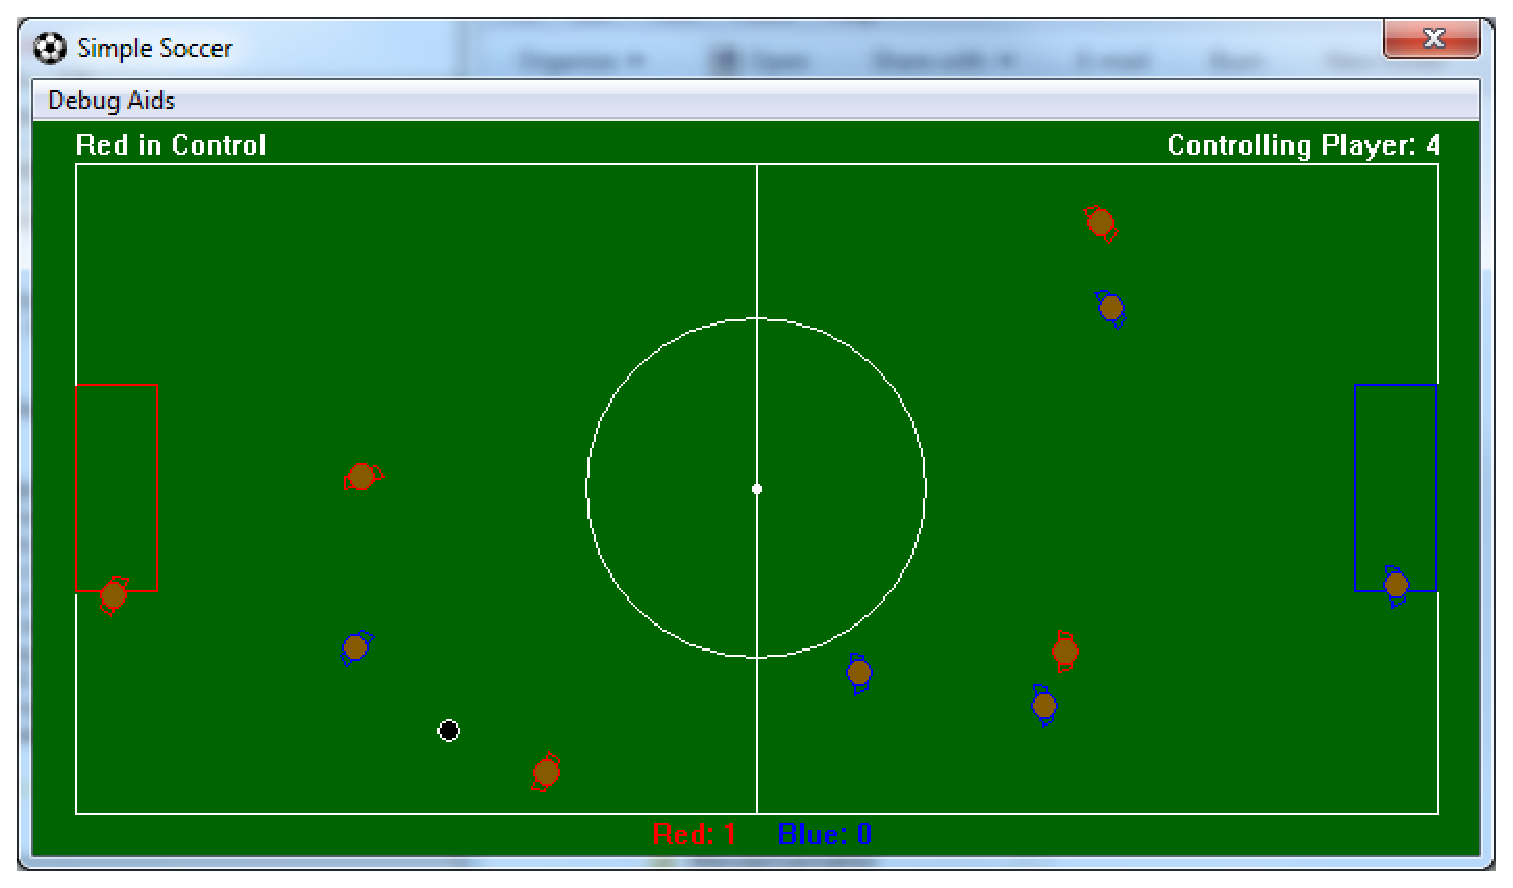
\includegraphics[scale=0.4]{simplesoccergame.eps}
\end{frame}

\bframe{Field Player Motion}
\bi
\li Uses speed and velocity-aligned heading unit vector
\li Heads track ball for illusion of intelligence
\bi\li Nobody receives ball from behind \ei
\li Uses steering behaviors
\bi\li arrive\li seek\li pursuit\ei
\ei
\end{frame}

\bframe{Field Player States}
\begin{itemize}
\item GlobalPlayerState (sends and receives messages)
\item Wait
\item ReceiveBall
\item KickBall
\item Dribble
\item ChaseBall
\item ReturnToHomeRegion
\item SupportAttacker
\end{itemize}
\end{frame}

\bframe{Messages for GlobalPlayerState}
\begin{itemize}
\item SupportAttacker
\item GoHome
\item ReceiveBall
\item PassToMe
\item Wait
\end{itemize}
\end{frame}

\bframe{ChaseBall}
\begin{itemize}
\item {\bf seek} the ball
\item Changes to KickBall if ball comes in range
\item Changes to ReturnToHomeRegion if not closest player to ball
\end{itemize}
\end{frame}

\bframe{Wait}
\begin{itemize}
\item If upfield of Controller, sends message PassToMe
\item If closest to ball, and no receiver, change to ChaseBall
\end{itemize}
\end{frame}

\bframe{ReceiveBall}
\begin{itemize}
\item Entered on message ReceiveBall
\item Only one player in ReceiveBall state
\item Uses either {\bf arrive} or {\bf pursuit} based on
\begin{itemize}
\item Randomness
\item Threatening opponent
\item Receiver close to opponent's goal
\end{itemize}
\item Change to ChaseBall if
\begin{itemize}
\item Ball comes close
\item Team loses control
\end{itemize}
\end{itemize}
\end{frame}

\bframe{KickBall}
\begin{itemize}
\item Change to ChaseBall when:
\begin{itemize}
\item Too soon after kick
\item Ball behind player
\item Player waiting to receive ball
\item Goalie has ball
\end{itemize}
\item If player has a shot, or occasionally randomly (potshots):
\begin{itemize}
\item Shoot ball with random noise added
\item Strength of kick determined by angle from player's heading
\item Change to Wait
\item Find support
\end{itemize}
\item If pass is possible and threatened:
\begin{itemize}
\item Pass ball with random noise added
\item Send message to receiver
\item Change to Wait
\item Find support
\end{itemize}
\item Otherwise, Find Support and change to Dribble
\end{itemize}
\end{frame}

\bframe{Dribble}
\begin{itemize}
\item Set controlling player to me
\item If ball is downfield, make small angled kicks
\item Otherwise kick upfield
\item Enter ChaseBall
\end{itemize}
\end{frame}

\bframe{SupportAttacker}
\begin{itemize}
\item {\bf arrive} at best support spot
\item If team loses the ball, change to ReturnToHomeRegion
\item If can shoot, send RequestPass to controlling player
\item If at best support spot:
\begin{itemize}
\item Steering off
\item Track ball
\item If not threatened, send RequestPass
\end{itemize}
\end{itemize}
\end{frame}

\bframe{Goalkeepers}
\begin{itemize}
\item Always faces ball
\item Moves laterally in front of the goal and along heading axis
\item States:
\begin{itemize}
\item GlobalKeeperState
\item TendGoal
\item ReturnHome
\item PutBallBackInPlay
\item InterceptBall
\end{itemize}
\end{itemize}
\end{frame}

\bframe{GlobalKeeperState}
\begin{itemize}
\item Receive message GoHome
\item Receive message ReceiveBall
\end{itemize}
\end{frame}

\bframe{TendGoal}
\begin{itemize}
\item {\bf interpose} between ball and a corresponding position in the goal
\item If ball is very close:
\begin{itemize}
\item Trap ball
\item Set GoalKeeperHasBall to true
\item Change state to PutBallBackInPlay
\end{itemize}
\item If ball is somewhat close:
\begin{itemize}
\item Change state to InterceptBall
\end{itemize}
\item If too far from goal:
\begin{itemize}
\item Change state to ReturnHome
\end{itemize}
\end{itemize}
\end{frame}

\bframe{ReturnHome}
\begin{itemize}
\item {\bf arrive} at home region
\item If in home region or team loses the ball:
\begin{itemize}
\item Change to TendGoal
\end{itemize}
\end{itemize}
\end{frame}

\bframe{PutBallBackInPlay}
\begin{itemize}
\item Set the controlling player to me
\item Message all field players on both teams to return home
\item If pass is available:
\begin{itemize}
\item Kick the ball
\item Set GoalKeeperHasBall to false
\item Send message ReceiveBall
\item Change to TendGoal
\end{itemize}
\end{itemize}
\end{frame}

\bframe{InterceptBall}
\begin{itemize}
\item {\bf pursuit} of ball
\item If too far from goal and goalie is NOT closest to the ball:
\begin{itemize}
\item Change to ReturnHome
\end{itemize}
\item If ball is very close:
\begin{itemize}
\item Trap the ball
\item Set GoalKeeperHasBall to true
\item Change to PutBallBackInPlay
\end{itemize}
\end{itemize}
\end{frame}

\bframe{isPassSafeFromOpponent}
\begin{itemize}
\item Yes if Opponent is behind player or farther back from target
  than receiver
\end{itemize}
\includegraphics[scale=0.25]{behind.png}
\end{frame}

\bframe{isPassSafeFromOpponent}
\begin{itemize}
\item Can opponent get to closest intercept point in time?
\end{itemize}
\includegraphics[scale=0.25]{closest.png}
\end{frame}

\bframe{CanShoot}
\begin{itemize}
\item Randomly pick several points along the goal line
\item Check each one to see if opponent can intercept
\end{itemize}
\end{frame}

\bframe{FindPass}
\begin{itemize}
\item Iterate through teammates within passing distance
\item Call GetBestPassToReceiver
\item Keep the one closest to goal
\end{itemize}
\end{frame}

\bframe{GetBestPassToReceiver}
\begin{itemize}
\item Calculate how long it takes ball to get to receiver
\item Find a circle one-third the size of receiver's range
\item Keep safe pass closest to goal
\end{itemize}
\includegraphics[scale=0.25]{bestpass.png}
\end{frame}

\bframe{Making Estimates and Assumptions}
\begin{itemize}
\item Artificial stupidity
\item It's more realistic
\item Two ways:
\begin{itemize}
\item Make it perfect and then dumb it down
\item Design it using simplifying assumptions
\end{itemize}
\item Examples:
\begin{itemize}
\item Adding random noise to a perfect kick
\item Using one-third size circles to estimate a receiver's range
\end{itemize}
\end{itemize}
\end{frame}

\end{document}


